\chapter{Anwendungen}
\label{cha:anwendungen}
% 6 Seiten

In den vergangen Jahren haben sich Unternehmen zunehmend an vielschichtigen neuronalen Netzten interessiert. Firmen wie Google\todo{einstellung ref}, Apple\todo{link} und Microsoft stellten renommierte Wissenschaftler ein und kaufen Unternehmen in diesem Bereich.

\subsection{Google Projekt}

In einem Projekt\todo{http://research.google.com/archive/unsupervised\_icml2012.html} 2012 trainierte Google ein Netz mit 10 Millionen Bilder aus dem Internet. Ein paar Eckdaten dazu:

\begin{figure}%
\centering
\subfloat[menschliches Gesicht]{\begin{minipage}{0.33\textwidth}\centering%
	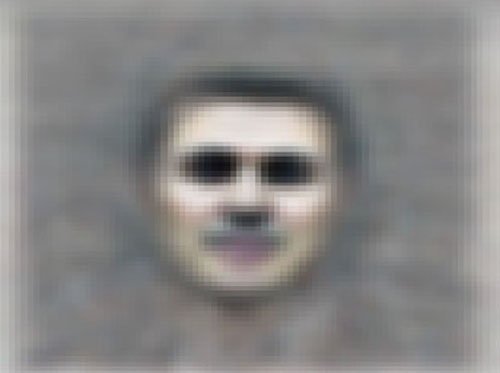
\includegraphics[width=0.9\textwidth]{images/neuron-face.jpg}\end{minipage}}
\subfloat[Gesicht einer Katze]{\begin{minipage}{0.33\textwidth}\centering%
	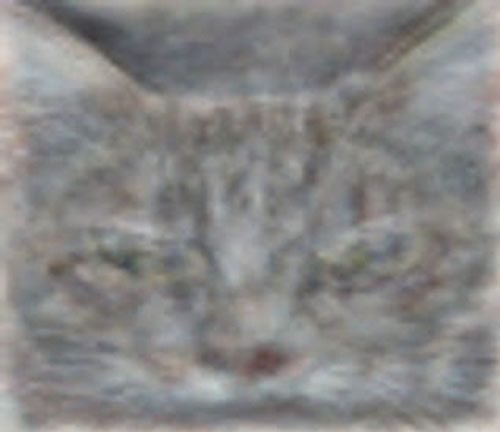
\includegraphics[width=0.9\textwidth]{images/neuron-cat.jpg}\end{minipage}}
\subfloat[menschlicher Körper]{\begin{minipage}{0.33\textwidth}\centering%
	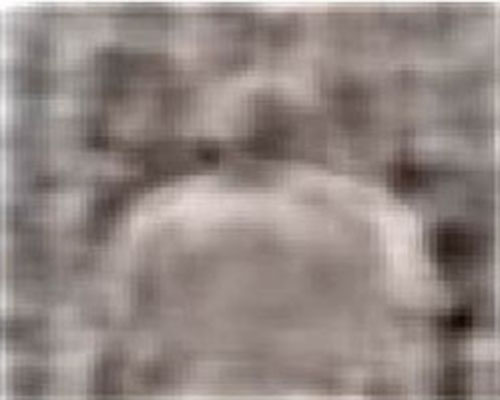
\includegraphics[width=0.9\textwidth]{images/neuron-body.jpg}\end{minipage}}
\caption{Markante Ausprägungen durch das lernen von Bildern aus dem Internet}
\label{fig:neurons-google}
\end{figure}

\begin{itemize}
\item 10 Millionen Trainingsbilder mit je 200x200 Pixel
\item Autoencoder mit sparse coding
\item 9 versteckte Schichten
\item 1 Milliarde Verbindungen
\item Training mit asynchronem stochastischem Gradientenvefahren
\item Auf auf 1000 Maschinen mit jeweils 16 Rechenkernen drei Tage lang trainiert
\end{itemize}

Bekannt wurde das Projekt vor allem durch die Ausprägung des in Abbildung \ref{} zu sehenden Gesichts- und Katzen-Neurons.
Es wurde mit relativ kleinen Bildern, dafür aber mit sehr vielen unbeaufsichtigt trainiert. Ein späterer Benchmark auf ImageNET, eine Datenbank mit Kategorisierten Bildern, ergab 15.8\% Trefferquote, das entspricht einer Steigerung des Spitzenwertes um 70\%.

Aus technischer Perspektive ist, die das Netz und damit die verwendete Technik weniger herausragend als die Menge der Trainingsdaten und die damit verbunden Rechenleistung.

%google autoencoder, https://www.youtube.com/watch?v=g4ZmJJWR34Q  23:54
%36:00 L2 polling, ignoriert dass ein neuron invertiert ausgelößt wird, zählt alles + auch wenn negativ, da die welt/bilder auch immer verdreht und manipuliert daher kommt, sprache muss akzente ignorieren, gesichtserkennung die haarfarbet etc. auf der richtigen ebene an Features ist das daher ein sehr nützlicher faktor}
%\todo[inline]{local constrast normalization, hilft auch bilder invariationen zu ignorieren}
%\todo[inline]{google hat mit obrigen in den letzten jahren viel in der Bildersuche und youtube erreicht - was genau?, unsupervised learning mit einer unmänge an daten aus youtube videos}
%\todo[inline]{44:46+ bild: stages, drei stages mit jeweils in reihe: filtering, l2 polling, lcn (normalization step) - am ende haben einige neuronen muster erkannt, eines feuert bei gesichtern, eines bei katzen}
%\todo[inline]{49:02 number of parameters: 1 billion ... 200x200px bilder, 18x18 filters, 8 filters per location, l2 polling and lcn over 5x5 neighborhoods - wie viele neuronen gesamt?}
%\todo[inline]{wegen rechenpower nur mit sehr wenig pixel (200x200) gerechnet, unsere augen sehen n x n pixel, noch einiges möglich}
%\todo[inline]{the input image that maximises the neuron to fire: 53:00, das neuron war auf der 3. ebene} 
%\todo[inline]{neuron auf 1. ebene sind edges, 2. ebene kombinationen von edges, 3. ebene muster wie das gesicht}
%\todo[inline]{IMAGENET, Datenbank mit gelabelten bildern an der sich viele Benchmarken}
%erkennt kanten da farben von der beleuchtung abhängen und somit varriieren
%lernen mittels back propagation

\section{Google Street View}

Google trainierte durch ihre Projekt Street View ein tiefes faltungskodiertes Netz das lernte Hausnummern zu erkennen. Für die Adresssuche auf Google Maps und dem damit verbundenen Navigationssystem ist es von wesentlicher Bedeutung Hausnummern richtig identifizieren zu können, besonders in Gebieten, bei denen Hausnummern nicht fortlaufend sind.

\todo{bild quelle: http://www.extremetech.com/computing/174275-google-has-built-a-neural-network-to-identify-100-million-house-numbers-for-streetview}

Google trainierte mehrere verschiedene Netze mit unterschiedlicher Anzahl an versteckten Schichten. Es stellte sich heraus, dass das tiefste Netz, mit elf versteckten Schichten die Hausnummern am besten erkennen konnte. Das Netz wurde mit über 100 Millionen hochauflösenden Bildern trainiert und forderte entsprechend viel Rechenleistung. Zum Training wurde daher der DistBelief\todo{link zu DistBelief algorithmus} Alogrithmus verwendet, ein Alogorithmus der sich besonders gut verteilt rechnen lässt. 

Nummern die das Netz nicht auflößen konnte, haben unbewusst Menschen gelöst. Hierzu hat Google ein Projekt ins Leben gerufen, das Besucher von Webseiten an sicherheitsrelevanten Stellen einen Code identifizieren lässt, um sicherzustellen dass es sich dabei tatsächlich um einen Menschen und keinen Bot handelt.

\begin{figure}
	\centering
	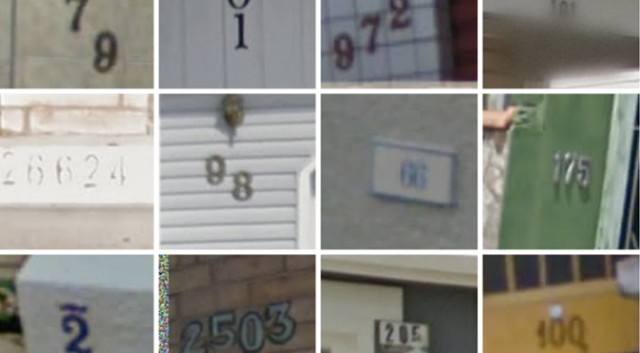
\includegraphics[width=0.7\textwidth]{images/streetview-numbers.jpg}
	\caption{Hausnummer die das neuronale Netz aus Google Street View erlernte.}
	\label{fig:streetview-numbers}
\end{figure}

Insgesamt hat das Netz bemerkenswert gut abgeschnitten\todo{http://arxiv.org/abs/1312.6082} und erkennt mittlerweile 97,84\% aller Hausnummern wie sie in Abbildung \ref{fig:streetview-numbers} zu sehen sind und sogar 99,8\% aller Sicherheitscodes der schwierigsten eingesetzten Art, der \emph{reCAPTCHA}\todo{}. Das Netz ist somit besser als die meisten Menschen, wodurch fraglich ist wie gut diese Sicherheitscodes in Zukunft tatsächlich vor Bots schützen werden.

\section{Spracherkennung}

Auch bei der Spracherkennung werden neuronale Netze in Kombination mit Deep Learning immer stärker und lösen nach und nach die Methode der Gaussian Mixture Models (GMM-Methoden) ab. Neuronale Netze für die Spracherkennung von Tonspuren funktionieren sehr ähnlich zu denen für die Bilderkennung. Wie bei der Bilderkennung prägen sich auf den ersten Schichten einfache Merkmale wie Konsonanten und Vokale aus. In höheren Schichten entstehen dann aussagekräftigere Merkmale bis hin zu vollständigen Wörtern, Phrasen und Stimmungen. 

Ein heute bereits aktives Feld der Anwendung ist die Sprachsteuerung von Geräten, die quasi auf allen großen Plattformen\todo{links siri, coratana, google now} verfügbar ist. Durch die große Menge an verfügbaren Sprachdaten von Mobiltelefonen, die zudem sehr gut kategorisierbar sind, ist zu erwarten, dass diese Netze in Zukunft noch stark an Bedeutung gewinnen werden.

\section{Hardware}

2012 Hat Google einen Rekord für das größte neuronale Netz, mit 1.000 Servern und 16.000 Rechenkernen aufgestellt. Bereits 2013 Hat NVIDIA\todo{referenz} gemeinsam mit der Stanford Universität ein 6,5-fach größeres neuronales Netz auf GPUs realisiert. Das Netz arbeitet auf nur 16 Computern mit jeweils vier Hochleistungs-Grafikkarten aus dem Konsumentenbereich und ist somit wesentlich günstiger.

Momentan entwickelt Qualcomm an Controller der eine neuronale Recheneinheit enthält. Der wesentliche Unterschied zu einer herkömmlichen CPU liegt dabei darin, dass alle Neuronen einer Schicht parallel rechnen. Das Netz benötigt daher nur wenige Zyklen bis zum Ergebnis, während herkömmliche CPUs jedes Neuron hintereinander berechnen muss. In den frühen Entwicklungsstufen konnte das Netz bereits einige Bilderkennungsaufgaben gleich gut wie komplexe mathematische Algorithmen lösen. Der Chip soll 2014 in die Massenproduktion gehen und unter anderem in Mobiltelefonen zur Verfügung stehen.

\section{Weitere Anwendungen}

\begin{tabular}{l l}
Verkehrsschilder erkennen & Traffic sign recognition (99,46prozenz, besser als menschen! gewinner http://www.kurzweilai.net/how-bio-inspired-deep-learning-keeps-winning-competitions)
\end{tabular}
